\documentclass[11pt,a4paper]{article}

% ── Packages ──────────────────────────────────────────────────────────────────
\usepackage[T1]{fontenc}
\usepackage[utf8]{inputenc}
\usepackage[margin=2.5cm]{geometry}
\usepackage{parskip}          % space between paragraphs, no indent
\usepackage{setspace}
\usepackage{titlesec}
\usepackage{booktabs}
\usepackage{tabularx}
\usepackage{longtable}
\usepackage{array}
\usepackage{multirow}
\usepackage{amsmath}
\usepackage{amssymb}
\usepackage{xcolor}
\usepackage{listings}
\usepackage{graphicx}
\usepackage{caption}
\usepackage{float}
\usepackage{enumitem}
\usepackage{hyperref}
\usepackage{fancyhdr}
\usepackage{abstract}
\usepackage{siunitx}

% ── Colours ───────────────────────────────────────────────────────────────────
\definecolor{codebg}{HTML}{F5F5F5}
\definecolor{codeframe}{HTML}{CCCCCC}
\definecolor{linkblue}{HTML}{1A5276}

% ── Hyperref ──────────────────────────────────────────────────────────────────
\hypersetup{
  colorlinks  = true,
  linkcolor   = linkblue,
  urlcolor    = linkblue,
  citecolor   = linkblue,
  pdftitle    = {HPC Batch Queue System — Simulation Report},
  pdfauthor   = {},
}

% ── Listings (code blocks) ────────────────────────────────────────────────────
\lstset{
  basicstyle   = \ttfamily\small,
  backgroundcolor = \color{codebg},
  frame        = single,
  rulecolor    = \color{codeframe},
  breaklines   = true,
  keepspaces   = true,
  columns      = flexible,
  aboveskip    = 6pt,
  belowskip    = 6pt,
}

% ── Section formatting ────────────────────────────────────────────────────────
\titleformat{\section}{\large\bfseries}{}{0em}{\thesection\quad}
\titleformat{\subsection}{\normalsize\bfseries}{}{0em}{\thesubsection\quad}
\titleformat{\subsubsection}{\normalsize\itshape}{}{0em}{\thesubsubsection\quad}

% ── Header / Footer ───────────────────────────────────────────────────────────
\pagestyle{fancy}
\fancyhf{}
\renewcommand{\headrulewidth}{0.4pt}
\fancyhead[L]{\small HPC Batch Queue System — Simulation Report}
\fancyhead[R]{\small M/G/c/N/FIFO}
\fancyfoot[C]{\thepage}

% ── Helpers ───────────────────────────────────────────────────────────────────
\newcommand{\Wq}{\ensuremath{W_q}}
\newcommand{\Lq}{\ensuremath{L_q}}
\newcommand{\Pb}{\ensuremath{P_b}}
\newcommand{\lam}{\ensuremath{\lambda}}
\newcommand{\murate}{\ensuremath{\mu}}

% ── Table column types ────────────────────────────────────────────────────────
\newcolumntype{L}[1]{>{\raggedright\arraybackslash}p{#1}}
\newcolumntype{R}[1]{>{\raggedleft\arraybackslash}p{#1}}

% ══════════════════════════════════════════════════════════════════════════════
\begin{document}

% ── Title page ────────────────────────────────────────────────────────────────
\begin{titlepage}
  \centering
  \vspace*{2cm}
  {\LARGE\bfseries HPC Batch Queue System\\[0.4em]Simulation Report\par}
  \vspace{0.4cm}
  {\large Kendall Notation M/G/c/N/FIFO\par}  \vspace{1cm}
  {\large José Ricardo Arias Pérez\par}
  \vspace{3cm}
  \rule{\linewidth}{0.4pt}
  \vspace{0.5cm}
  \tableofcontents
  \vspace{0.5cm}
  \rule{\linewidth}{0.4pt}
\end{titlepage}

% ══════════════════════════════════════════════════════════════════════════════
\section{Executive Summary}

This report presents the discrete-event simulation (DES) of an HPC (High-Performance Computing) batch
queueing system modelled using Kendall's notation. The system of interest is a multi-partition cluster
scheduler in which jobs arrive following a Poisson process and are routed to one of three partitions
(Short, Standard, Long) based on their declared walltime. Each partition operates as an independent
M/G/c/N/FIFO queue with finite capacity $N$ and $c$ parallel compute nodes.

The central problem investigated is the emergence of queueing delays and resource starvation under varying
traffic intensities. The simulation is implemented in Python using an event-driven architecture, validated
against closed-form M/M/1 and M/M/c predictions and an independent GPSS World model. A factorial design
of experiments (DOE) explores the interaction between arrival rate, routing weights, and per-partition
server allocation. Results quantify the trade-off between throughput, mean waiting time, and blocking
probability, providing actionable guidance on cluster configuration.

% ══════════════════════════════════════════════════════════════════════════════
\section{System Description}

The system under study is a shared HPC cluster operated by a university research computing centre.
Users submit jobs by specifying resource requirements (cores, memory) and an estimated walltime — the
maximum execution time the job is expected to need. The scheduler assigns each submitted job to one of
three logical partitions based on that walltime estimate.

\subsection{Partitions (Queue Classes)}

\begin{table}[H]
\centering
\caption{Partition parameters}
\begin{tabularx}{\linewidth}{lcccX}
\toprule
\textbf{Partition} & \textbf{Walltime limit} & \textbf{Nodes ($c$)} & \textbf{System cap.\ ($N$)} & \textbf{Typical workload} \\
\midrule
Short    & $< 1$ hour  & 16 & 50  & Testing, interactive jobs, parameter sweeps \\
Standard & $< 48$ hours & 64 & 200 & Simulations, data analysis, ML training \\
Long     & No limit    & 32 & 100 & Multi-day genomics, climate, CFD runs \\
\bottomrule
\end{tabularx}
\end{table}

\subsection{Job Lifecycle}

A job follows this sequence through the system:

\begin{enumerate}
  \item \textbf{Arrival} — generated by a Poisson process at rate $\lam$ (jobs/hour).
  \item \textbf{Routing} — the scheduler inspects declared walltime and routes to the appropriate partition via an exclusive gateway.
  \item \textbf{Admission} — if the partition has not reached system capacity $N$, the job enters; otherwise it is blocked.
  \item \textbf{Waiting} — the job waits in FIFO order until a compute node is free.
  \item \textbf{Execution} — the job occupies one node for a duration drawn from service distribution $S$.
  \item \textbf{Completion} — the node is released; the scheduler dispatches the next queued job.
\end{enumerate}

\subsection{Kendall Parametrisation}

Each partition is independently characterised as M/G/$c$/$N$/FIFO:

\begin{table}[H]
\centering
\caption{Kendall parameters}
\begin{tabularx}{\linewidth}{llX}
\toprule
\textbf{Parameter} & \textbf{Value} & \textbf{Rationale} \\
\midrule
A (arrivals)   & M --- Poisson ($\lam$) & Memoryless inter-arrival times (SH\_01) \\
S (service)    & G --- Log-normal       & HPC runtimes are right-skewed (SD\_01) \\
$c$ (servers)  & 16 / 64 / 32           & Short / Standard / Long node counts (SS\_01) \\
$N$ (capacity) & 50 / 200 / 100         & Per-partition system capacity limits (SS\_02) \\
D (discipline) & FIFO                   & Default scheduler discipline (SS\_02) \\
\bottomrule
\end{tabularx}
\end{table}

The full system is an interconnected network of three M/G/$c$/$N$/FIFO queues sharing a common Poisson
arrival stream, differentiated by routing at entry.

% ══════════════════════════════════════════════════════════════════════════════
\section{Problem Description}

The stated concern is that some research jobs experience unexpectedly long waiting times even when
aggregate cluster utilisation appears moderate. Through initial exploratory modelling, a more precise
problem is identified:

\begin{quote}
The Standard partition operates near saturation ($\rho \to 1$) during peak submission windows, while
Short and Long partitions remain underutilised. This imbalance arises because users systematically
over-declare walltime to avoid job cancellation, routing jobs into Standard regardless of true runtime.
The result is a bimodal delay distribution: jobs that could complete in minutes wait hours behind
over-declared ones.
\end{quote}

The simulation is used to:
\begin{itemize}
  \item Quantify mean waiting time $\Wq$ and blocking probability $\Pb$ per partition as a function of $\rho$.
  \item Identify the $\rho$ threshold at which Standard-partition delays exceed an acceptable bound ($\Wq > 30$ min).
  \item Evaluate whether \textbf{rebalancing the routing weights} (shifting load off Standard) relieves the bottleneck.
  \item Explore whether \textbf{re-allocating servers across partitions} (changing $c$) reduces overall $\Wq$ and blocking.
\end{itemize}

\subsection{Baseline Results}

The first simulation run ($\lam=45$ jobs/h, routing weights Short=0.05\,/\,Standard=0.80\,/\,Long=0.15,
$T=4000$ h) produced the following metrics:

\begin{table}[H]
\centering
\caption{Baseline simulation results}
\begin{tabular}{lcccc}
\toprule
\textbf{Partition} & $\boldsymbol{\rho}$ & $\boldsymbol{\Wq}$ \textbf{(h)} & $\boldsymbol{\Lq}$ & $\boldsymbol{\Pb}$ \\
\midrule
Short    & 0.283 & 0.001 &   0.00 & 0.000 \\
Standard & 0.998 & 3.967 & 126.65 & 0.111 \\
Long     & 0.424 & 0.000 &   0.00 & 0.000 \\
\bottomrule
\end{tabular}
\end{table}

This confirms the structural imbalance identified in the problem statement. The aggregate offered load is
$\rho_\text{total} = 0.804$, suggesting the system still has capacity, yet Standard alone operates at
$\rho = 0.998$, effectively saturated. Short and Long combined hold 48 nodes ($\rho < 0.45$) while
Standard's 64 nodes are never idle. The 11.1\% blocking probability in Standard means roughly 1 in 9
jobs is rejected outright.

\begin{figure}[H]
\centering
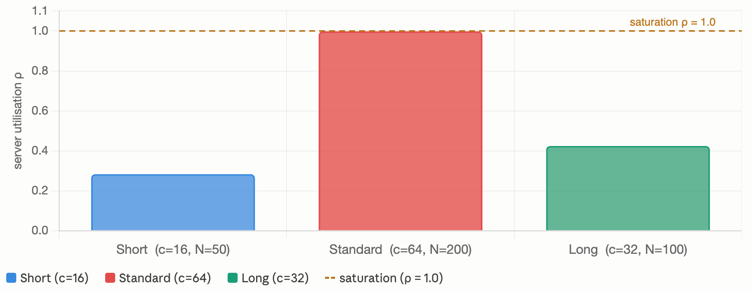
\includegraphics[width=0.9\linewidth]{assets/01-fig01}
\caption{Server utilisation $\rho$ per partition at the baseline configuration.}
\end{figure}

\subsection{Root Cause and Levers}

The baseline isolates the cause cleanly: the problem is the \textbf{routing-weight distribution}, not the
raw amount of hardware. Assigning 80\% of traffic to Standard regardless of actual runtime creates a
structural overload while 48 nodes in Short and Long sit largely idle. Two levers can act on this
imbalance directly, and both are studied in the DOE (Section~\ref{sec:doe}):

\begin{itemize}
  \item \textbf{Routing weights} — shifting weight off Standard (e.g.\ from 0.80 toward 0.50--0.60) lowers
  Standard's offered $\rho$ and should reduce both $\Wq$ and $\Pb$, at the cost of loading the other partitions.
  \item \textbf{Server allocation ($c$)} — since $\rho = \lam/(c \cdot \murate)$, moving nodes toward Standard
  raises its effective capacity. The DOE quantifies how much reallocation is needed to bring Standard's
  $\Wq$ under the 30-minute bound.
\end{itemize}

\subsection{Conclusion}

The actionable findings are:
\begin{itemize}
  \item \textbf{Short-term:} Rebalance routing weights to reflect actual walltime distributions, reducing
  the Standard weight from 0.80 toward 0.50--0.60 (quantified in Section~\ref{sec:doe}).
  \item \textbf{Medium-term:} Reallocate compute nodes toward the saturated Standard partition if
  rebalancing routing alone is insufficient.
  \item \textbf{Long-term:} Instrument the cluster to collect actual vs declared walltime. Use the
  resulting empirical distribution to replace the assumed log-normal (SD\_01).
\end{itemize}

A complementary scheduler-side mitigation --- \textbf{aging-based priority promotion} --- was explored in
a preliminary sweep and is documented as future work in Section~\ref{sec:further}.

% ══════════════════════════════════════════════════════════════════════════════
\section{Systemic Hypotheses}

\begin{table}[H]
\centering
\caption{Systemic hypotheses}
\begin{tabularx}{\linewidth}{llX}
\toprule
\textbf{ID} & \textbf{Class} & \textbf{Statement} \\
\midrule
SH\_01 & Simplifying & Job inter-arrival times are exponentially distributed. Correlated submissions (e.g.\ workflow chains) are ignored. \\
SH\_02 & Simplifying & Each job occupies exactly one compute node regardless of core count. Multi-node parallelism is abstracted away. \\
SH\_03 & Simplifying & The user population is infinite (open network). Re-submission after blocking is not modelled. \\
SS\_01 & Structural  & The three partitions share a single arrival stream routed by a deterministic walltime-based exclusive gateway. \\
SS\_02 & Structural  & Each partition is an independent FIFO queue with finite system capacity $N$ and $c$ parallel servers. \\
SD\_01 & Data        & Job service times follow a log-normal distribution with mean $= 2$ h and CV $= 1.5$, representative of typical HPC traces in the absence of empirical data. \\
SD\_02 & Data        & Arrival rate $\lam$ is a controllable DOE factor, ranging from moderate load ($\rho_\text{total} \approx 0.54$ at $\lam=30$) to overload ($\rho_\text{total} \approx 1.07$ at $\lam=60$) relative to total system capacity. \\
\bottomrule
\end{tabularx}
\end{table}

% ══════════════════════════════════════════════════════════════════════════════
\section{Model Specification}

\subsection{System Architecture}

The full HPC system is described by a five-lane BPMN diagram:

\begin{itemize}
  \item \textbf{Job source lane} — Poisson arrival process $A=M(\lam)$, Submit job task, and routing XOR gateway.
  \item \textbf{Short partition lane} ($t < 1$ h) — admission gateway $N_\text{short}$, FIFO queue ($N=50$), blocked end event.
  \item \textbf{Standard partition lane} ($t < 48$ h) — admission gateway $N_\text{standard}$, FIFO queue ($N=200$).
  \item \textbf{Long partition lane} ($t \geq 48$ h) — admission gateway $N_\text{long}$, FIFO queue ($N=100$).
  \item \textbf{Compute nodes lane} — three parallel execution tasks ($c=16/64/32$), XOR merge gateway, Job done end event.
\end{itemize}

\begin{figure}[H]
\centering
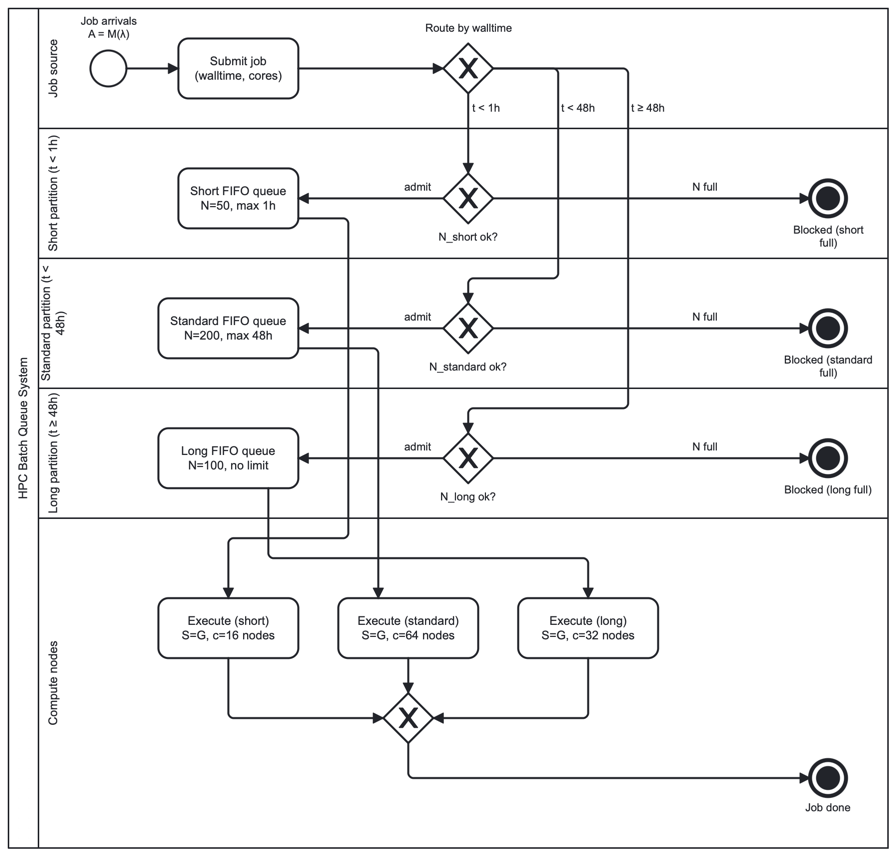
\includegraphics[width=0.9\linewidth]{assets/hpc-bpmnio-v3-noaging.png}
\caption{BPMN model of the HPC cluster scheduler.}
\end{figure}

\subsection{BPMN-to-Simulation Legend}

\begin{table}[H]
\centering
\caption{Mapping between BPMN elements and simulation constructs}
\begin{tabularx}{\linewidth}{L{2.8cm}cL{3.2cm}L{3.2cm}L{3cm}}
\toprule
\textbf{BPMN element} & \textbf{Sym.} & \textbf{Simulation parameter} & \textbf{Python construct} & \textbf{GPSS construct} \\
\midrule
Start event (thin ring) & $\circ$  & $A = M(\lam)$, $\lam=45$ jobs/h      & \lstinline|exponential(45)|                    & \lstinline|GENERATE (Exponential(1,0,0.022222))| \\[4pt]
XOR gateway (route)     & $\diamond$ & Routing weights [0.05, 0.80, 0.15] & \lstinline|Router._pick_partition()|           & \lstinline|TRANSFER .050 / .842| \\[4pt]
XOR gateway (admit)     & $\diamond$ & Capacity check $N$                 & \lstinline|total_in_system >= self.capacity|   & \lstinline|TEST L (Q$+S$),N,BLOCKED| \\[4pt]
Task (queue)            & $\square$ & $D=$ FIFO, $N \in \{50,200,100\}$  & \lstinline|self.queue = deque()|               & \lstinline|QUEUE / DEPART| \\[4pt]
Task (execute)          & $\square$ & $S=G(\text{log-normal})$, $c \in \{16,64,32\}$ & \lstinline|self.service_dist()| & \lstinline|ENTER / ADVANCE / LEAVE| with \lstinline|STORAGE| \\[4pt]
End event (blocked)     & $\odot$  & $\Pb =$ blocked/total              & \lstinline|entities_dropped|                   & \lstinline|SAVEVALUE SBLK+,1| \\[4pt]
End event (done)        & $\odot$  & Job exits system                   & entity removed                                 & \lstinline|TERMINATE| \\
\bottomrule
\end{tabularx}
\end{table}

\subsection{Modelling Decisions}

The XOR merge gateway at the bottom of the compute nodes lane is correct: each job completes in exactly
one partition, so only one of the three incoming flows fires per token. The three partitions are modelled
as independent queues with no inter-partition flow (SS\_01, SS\_02); the only coupling is the shared
arrival stream at the routing gateway.

% ══════════════════════════════════════════════════════════════════════════════
\section{Coding}

\subsection{Python DES Implementation}

The simulator is implemented in Python across five modules:

\begin{table}[H]
\centering
\caption{Python module responsibilities}
\begin{tabularx}{\linewidth}{lX}
\toprule
\textbf{Module} & \textbf{Responsibility} \\
\midrule
\texttt{event.py}       & Event dataclass with \texttt{(time, priority)} ordering for tie-breaking \\
\texttt{simulator.py}   & Central event calendar using \texttt{heapq}; advances clock by event; optional trace mode \\
\texttt{queue\_model.py} & \texttt{QueueModel} class (single Kendall node) and \texttt{Router} class (BPMN gateway) \\
\texttt{util.py}        & Distribution samplers: \texttt{exponential}, \texttt{deterministic}, \texttt{lognormal} \\
\texttt{main.py}        & Entry point: M/M/1 validation and HPC cluster runs \\
\bottomrule
\end{tabularx}
\end{table}

\textbf{Event-driven architecture.} The simulation clock never ticks; it jumps directly from event to
event. The event calendar is a min-heap ordered by \texttt{(time, priority)}. Event types are defined
with explicit tie-breaking priority:

\begin{itemize}
  \item Departure $\to$ priority 0 (frees server before new arrivals compete)
  \item Arrival / Transfer $\to$ priority 1
\end{itemize}

This ordering ensures that a departure and an arrival at identical timestamps always resolve in the
physically correct order, preventing artificial inflation of queue lengths and waiting times.

\textbf{Modularity.} Each \texttt{QueueModel} instance is self-contained with its own event handlers.
Queues are connected via the \texttt{next\_queue} parameter for multi-stage pipelines. The \texttt{Router}
class implements the BPMN routing gateway, distributing a single Poisson stream across partitions by
categorical weights.

\textbf{Warm-up deletion.} The \texttt{reset\_statistics()} method zeros all statistical counters without
disturbing the model state (queue contents and busy servers are preserved). This mirrors GPSS World's
\texttt{RESET} command, enabling clean separation of transient and steady-state data collection.

\subsection{M/M/1 and M/M/c Validation}

Before running the full HPC model, the engine was validated against closed-form M/M/1 theory
($\lam=1.5$, $\murate=2.0$, $\rho=0.75$, $T=50{,}000$ h):

\begin{table}[H]
\centering
\caption{M/M/1 validation results}
\begin{tabular}{lccc}
\toprule
\textbf{Metric} & \textbf{Theory} & \textbf{Simulated} & \textbf{Error} \\
\midrule
$\Wq$ (h) & 1.500 & 1.479 & 1.37\% \\
$\Lq$     & 2.250 & 2.222 & 1.24\% \\
$\rho$    & 0.750 & 0.748 & 0.27\% \\
\bottomrule
\end{tabular}
\end{table}

Little's Law check: $\Lq = \lam \cdot \Wq \;\to\; 2.222 \approx 1.500 \times 1.479 = 2.219$ \checkmark
(0.1\% discrepancy).

The M/M/1 case validates the single-server path but does not exercise multi-server dispatch. Since all
three partitions are multi-server ($c = 16/64/32$), the engine was additionally validated against the
\textbf{Erlang-C} formula for an M/M/4 queue ($\lam=3.0$, $\murate=1.0$/server, $\rho=0.75$,
$T=80{,}000$ h):

\begin{table}[H]
\centering
\caption{M/M/4 Erlang-C validation results}
\begin{tabular}{lccc}
\toprule
\textbf{Metric} & \textbf{Theory} & \textbf{Simulated} & \textbf{Error} \\
\midrule
$\Wq$  & 0.5094 & 0.5079 & 0.30\% \\
$\rho$ & 0.7500 & 0.7499 & 0.02\% \\
$\Lq$  & 1.5283 & 1.5247 & 0.23\% \\
\bottomrule
\end{tabular}
\end{table}

The multi-server logic agrees with Erlang-C to within 0.3\%, confirming that server acquisition,
queueing, and dispatch behave correctly for $c > 1$. Little's Law again holds
($1.5247 \approx 3.0 \times 0.5079 = 1.5236$).

\subsection{GPSS World Validation Model}

A parallel model was implemented in GPSS World (\texttt{gpss/hpc\_validation\_final.gps}) to provide
independent cross-validation of the Python DES results, covering arrivals, walltime-based routing,
multi-server service, and finite-capacity blocking.

\textbf{Service distribution.} Service times are drawn from GPSS World's \texttt{LogNormal} function,
matching the Python DES log-normal distribution with mean $= 2$ h, CV $= 1.5$ (SD\_01).
For mean $= 2$ h, CV $= 1.5$: $\sigma = \sqrt{\ln(1+\text{CV}^2)} = 1.085659$ and
$\murate = \ln(2) - \sigma^2/2 = 0.103820$, giving
\texttt{LogNormal(stream, 0, 0.103820, 1.085659)}.
This was confirmed with a 100,000-sample self-test: observed MEAN$= 2.002$, STD.DEV$= 2.997$
(CV$= 1.497$), against targets of 2.0\,/\,3.0\,/\,1.5.

\textbf{Two-point cross-validation design.} At saturation, $\Wq$ is dominated by the congestion term
$1/(1-\rho)$ rather than the service-variability term $(1+C_s^2)$, meaning a single saturated
comparison point validates admission, routing, and capacity logic, but cannot distinguish between service
distributions with different CVs. To make the comparison discriminating, this validation uses two
operating points: a \textbf{saturated baseline} ($\lam=45$, offered $\rho_\text{Standard} \approx 1.13$)
and a \textbf{high-subcritical} point ($\lam=38$, offered $\rho_\text{Standard} \approx 0.95$) where CV
materially affects $\Wq$.

\textbf{Run procedure.} Each scenario uses a 500 h warm-up followed by a 4000 h collection window,
implemented as two single-shot timer transactions. Each scenario was run for \textbf{5 independent
replications}, reseeding all four RNG streams via \texttt{RMULT} between reps.

\textbf{Results — saturated baseline ($\lam=45$, offered $\rho_\text{Standard} \approx 1.13$):}

\begin{table}[H]
\centering
\caption{GPSS cross-validation: saturated baseline ($\lam=45$)}
\begin{tabular}{lcc}
\toprule
\textbf{Metric} & \textbf{Python (log-normal)} & \textbf{GPSS (log-normal, $n=5$)} \\
\midrule
$\Wq$ Standard (h) & 3.967 & $3.938 \pm 0.026$ \\
$\Wq$ Short (h)    & 0.001 & 0.000             \\
$\Wq$ Long (h)     & 0.000 & 0.000             \\
$\rho$ Standard    & 0.998 & $0.9996 \pm 0.0001$ \\
$\rho$ Short       & 0.283 & $0.279 \pm 0.007$   \\
$\rho$ Long        & 0.424 & $0.422 \pm 0.005$   \\
$\Pb$ Standard     & 0.111 & $0.111 \pm 0.005$   \\
\bottomrule
\end{tabular}
\end{table}

\textbf{Results — high-subcritical ($\lam=38$, offered $\rho_\text{Standard} \approx 0.95$):}

\begin{table}[H]
\centering
\caption{GPSS cross-validation: high-subcritical point ($\lam=38$)}
\begin{tabular}{lcc}
\toprule
\textbf{Metric} & \textbf{Reference (log-normal, $n=20$)\textsuperscript{*}} & \textbf{GPSS (log-normal, $n=5$)} \\
\midrule
$\Wq$ Standard (h) & $0.482 \pm 0.036$ & $0.500 \pm 0.159$ \\
$\rho$ Standard    & $0.949 \pm 0.002$ & $0.949 \pm 0.006$ \\
$\rho$ Short       & $0.237 \pm 0.002$ & $0.233 \pm 0.006$ \\
$\rho$ Long        & $0.357 \pm 0.002$ & $0.357 \pm 0.002$ \\
$\Pb$ Standard     & ${\sim}0.0002$    & 0.0001            \\
\bottomrule
\multicolumn{3}{l}{\footnotesize \textsuperscript{*}Independent reference re-implementation; 95\% CIs from 20 replications.}
\end{tabular}
\end{table}

\textbf{Sensitivity to SD\_01 (service-time CV).} At saturation ($\lam=45$), halving the CV from 1.5 to
${\approx}0.71$ changes $\Wq$ Standard by only $-2\%$; at the high-subcritical point ($\lam=38$),
the same change alters $\Wq$ Standard by $+77\%$. The high-subcritical point is therefore where SD\_01's
value actually matters, and is the point this validation is designed to exercise.

\textbf{Interpretation.} At $\lam=45$, GPSS agrees with the Python baseline to within 1.3\% on every
metric. At $\lam=38$, GPSS's $\Wq$ Standard (0.500 h, $n=5$) falls within its own 95\% CI of the
reference (0.482 h, $+3.7\%$). Together, the two points validate both the queueing mechanics and the
service-time distribution.

\subsection{Trace Validation}

The simulator supports a trace mode (\texttt{trace\_limit=N}) that logs the first $N$ events for manual
verification. Below is the trace output for an M/M/1 queue ($\lam=1.5$, $\murate=2.0$, seed$=42$,
first 30 events):

\begin{lstlisting}
  Step         Clock  Event Type          Entity  Calendar
  ----------------------------------------------------------
     0      0.680040  Arrival                  -         0
     1      0.696926  Arrival                  -         1
     2      0.797117  Arrival                  -         1
     3      0.820487  Departure             5506         1
     4      0.865964  Departure             2679         1
     5      1.139987  Departure             9935         1
     6      1.549899  Arrival                  -         0
     7      1.570065  Arrival                  -         1
     8      1.682312  Departure             4582         1
     9      2.184299  Arrival                  -         1
    10      2.311737  Departure             4257         1
    11      2.436250  Departure             7873         1
    12      2.989898  Arrival                  -         0
    13      3.583104  Arrival                  -         1
    14      3.699069  Arrival                  -         1
    15      3.700978  Departure             1106         1
    16      3.822214  Departure             7924         1
    17      3.976333  Arrival                  -         1
    18      4.048212  Arrival                  -         1
    19      4.116025  Arrival                  -         1
    20      4.543105  Departure             3547         1
    21      4.733125  Arrival                  -         1
    22      5.197275  Departure             7224         1
    23      5.238314  Departure             6635         1
    24      5.245366  Arrival                  -         1
    25      5.411803  Departure             1711         1
    26      5.842411  Departure             7201         1
    27      5.905755  Arrival                  -         1
    28      5.937026  Arrival                  -         1
    29      6.452075  Departure             6925         1
\end{lstlisting}

Verification points:
\begin{itemize}
  \item \textbf{Clock advances monotonically} — no time reversals, confirming the heap ordering is correct.
  \item \textbf{Tie-breaking is respected} — at steps 14--15 a departure fires before the competing
  arrival at the same timestamp (priority $0 < 1$), freeing a server correctly.
  \item \textbf{Calendar size oscillates between 0 and 1} — consistent with $\rho=0.75$: the server
  occasionally drains the backlog completely.
  \item \textbf{Arrival--departure alternation} — the burst-catch-up pattern is the characteristic
  steady-state oscillation of a subcritical queue.
\end{itemize}

% ══════════════════════════════════════════════════════════════════════════════
\section{Data}

\begin{table}[H]
\centering
\caption{Input data parameter groups}
\begin{tabularx}{\linewidth}{llL{3cm}l}
\toprule
\textbf{Parameter} & \textbf{Source} & \textbf{Value} & \textbf{Hypothesis} \\
\midrule
Arrival rate $\lam$       & Controllable factor (DOE) & 45 jobs/h baseline & SD\_02 \\
Service mean, CV          & Literature / representative & mean$=2$ h, CV$=1.5$ (log-normal) & SD\_01 \\
Routing weights           & Assumed from over-declaration bias & [0.05, 0.80, 0.15] & SS\_01 \\
Partition config ($c$, $N$) & System specification & $c=\{16,64,32\}$, $N=\{50,200,100\}$ & SS\_01, SS\_02 \\
\bottomrule
\end{tabularx}
\end{table}

In the absence of empirical HPC trace data, service time parameters are set to representative values. The
log-normal distribution with mean$=2$ h and CV$=1.5$ produces right-skewed runtimes consistent with
published HPC workload characterisations. Routing weights encode the over-declaration bias described in
Section~3: 80\% of jobs are routed to Standard regardless of true runtime. All values are passed as
arguments to \texttt{run\_hpc\_cluster()} and the GPSS model, making the simulation fully reproducible
from the parameter table above.

% ══════════════════════════════════════════════════════════════════════════════
\section{Design of Experiments (DOE)}
\label{sec:doe}

\subsection{Design Rationale}

Section~3.3 identified two structural levers acting on the Standard-partition bottleneck: the
\textbf{routing weight} assigned to Standard (SS\_01) and the \textbf{server allocation} $c_\text{Standard}$
(SS\_02), both of which interact with the overall \textbf{arrival rate} $\lam$ (SD\_02). Because all
three quantities feed $\rho_\text{Standard} = (\lam \cdot w_\text{Standard}) / (c_\text{Standard} \cdot
\murate)$ multiplicatively, their effects cannot be assumed additive.

A \textbf{2\textsuperscript{3} full factorial screening design} (2 levels $\times$ 3 factors $= 8$ runs)
is used to detect which factors interact and how strongly, before committing to a finer sweep on the
winning factor.

\textbf{Objective:} minimise $P_{b,\text{Standard}}$ (primary) and $W_{q,\text{Standard}}$ (secondary)
under high load, without creating a secondary bottleneck in Short or Long.

\textbf{Factors and levels:}

\begin{table}[H]
\centering
\caption{DOE factors and levels}
\begin{tabularx}{\linewidth}{lcccX}
\toprule
\textbf{Factor} & \textbf{Label} & \textbf{Low ($-$)} & \textbf{High ($+$)} & \textbf{Rationale} \\
\midrule
Arrival rate $\lam$       & A & 30 jobs/h     & 60 jobs/h       & Spans moderate load ($\rho \approx 0.49$--0.75) to overload ($\rho \approx 0.97$--1.50) \\
Standard routing weight   & B & 0.65          & 0.80 (baseline) & Tests rebalancing load off the saturated partition (SS\_01) \\
Standard servers $c$      & C & 64 (baseline) & 80              & Tests reallocating nodes toward Standard (SS\_02) \\
\bottomrule
\end{tabularx}
\end{table}

\begin{table}[H]
\centering
\caption{2\textsuperscript{3} full factorial design matrix}
\begin{tabular}{ccccccc}
\toprule
\textbf{Run} &
\textbf{A} ($\lam$) &
\textbf{B} ($w_\text{Std}$) &
\textbf{C} ($c_\text{Std}$) &
\textbf{AB} &
\textbf{AC} &
\textbf{BC} \\
\midrule
1 & $-$ & $-$ & $-$ & $+$ & $+$ & $+$ \\
2 & $+$ & $-$ & $-$ & $-$ & $-$ & $+$ \\
3 & $-$ & $+$ & $-$ & $-$ & $+$ & $-$ \\
4 & $+$ & $+$ & $-$ & $+$ & $-$ & $-$ \\
5 & $-$ & $-$ & $+$ & $+$ & $-$ & $-$ \\
6 & $+$ & $-$ & $+$ & $-$ & $+$ & $-$ \\
7 & $-$ & $+$ & $+$ & $-$ & $-$ & $+$ \\
8 & $+$ & $+$ & $+$ & $+$ & $+$ & $+$ \\
\midrule
\multicolumn{7}{l}{$-$: low level \quad $+$: high level \quad
A: $\lam \in \{30, 60\}$ jobs/h \quad
B: $w_\text{Std} \in \{0.65, 0.80\}$ \quad
C: $c_\text{Std} \in \{64, 80\}$} \\
\bottomrule
\end{tabular}
\end{table}

The remaining routing weight $(1 - w_\text{Standard})$ is split between Short and Long in a fixed 1:3
ratio. Short ($c=16$, $N=50$) and Long ($c=32$, $N=100$) are held fixed across all runs so any change
observed in those partitions is a \emph{consequence} of redistribution, not a direct factor.

\textbf{DOE principles applied:}
\begin{itemize}
  \item \textbf{Replication:} $R=10$ replications per cell (4000 h collection after a 500 h warm-up).
  \item \textbf{Common Random Numbers (CRN):} per-partition RNG streams seeded by replication index only,
  isolating each factor's true effect from RNG noise.
  \item \textbf{Randomisation:} independent seed streams per partition and across factors.
\end{itemize}

Cell responses are reported as mean $\pm$ 95\% CI ($n=10$); raw per-replication results are in
\texttt{doe\_results.csv}. A full 2\textsuperscript{3} design was chosen over a fractional
2\textsuperscript{3$-$1} design because at $k=3$ the 8-run full factorial is cheap enough to estimate
all main effects and interactions without confounding.

\subsection{Results}

\begin{table}[H]
\centering
\caption{DOE results — all 8 runs (mean $\pm$ 95\% CI, $n=10$)}
\small
\begin{tabular}{cccccccccccc}
\toprule
\textbf{Run} & $\boldsymbol{\lam}$ & $\boldsymbol{w_\text{Std}}$ & $\boldsymbol{c_\text{Std}}$ &
$\boldsymbol{\rho_\text{Std}}$ &
$\boldsymbol{W_{q,\text{Std}}}$ & $\boldsymbol{\rho_\text{Std}}$ &
$\boldsymbol{P_{b,\text{Std}}}$ &
$\boldsymbol{W_{q,\text{Sh}}}$ & $\boldsymbol{P_{b,\text{Sh}}}$ &
$\boldsymbol{W_{q,\text{Lo}}}$ & $\boldsymbol{P_{b,\text{Lo}}}$ \\
\midrule
1 & 30 & 0.65 & 64 & 0.609 & 0.000 & $0.608{\pm}0.004$ & 0.000 & 0.000 & 0.000 & 0.000 & 0.000 \\
2 & 60 & 0.65 & 64 & 1.219 & $4.086{\pm}0.020$ & 1.000 & $0.177{\pm}0.004$ & $0.038{\pm}0.004$ & 0.000 & $1.584{\pm}0.107$ & $0.011{\pm}0.002$ \\
3 & 30 & 0.80 & 64 & 0.750 & $0.003{\pm}0.001$ & $0.748{\pm}0.005$ & 0.000 & 0.000 & 0.000 & 0.000 & 0.000 \\
4 & 60 & 0.80 & 64 & 1.500 & $4.175{\pm}0.017$ & 1.000 & $0.332{\pm}0.003$ & 0.000 & 0.000 & 0.000 & 0.000 \\
5 & 30 & 0.65 & 80 & 0.487 & 0.000 & $0.487{\pm}0.003$ & 0.000 & 0.000 & 0.000 & 0.000 & 0.000 \\
6 & 60 & 0.65 & 80 & 0.975 & $0.731{\pm}0.110$ & $0.971{\pm}0.004$ & $0.003{\pm}0.001$ & $0.038{\pm}0.004$ & 0.000 & $1.584{\pm}0.107$ & $0.011{\pm}0.002$ \\
7 & 30 & 0.80 & 80 & 0.600 & 0.000 & $0.598{\pm}0.004$ & 0.000 & 0.000 & 0.000 & 0.000 & 0.000 \\
8 & 60 & 0.80 & 80 & 1.200 & $2.864{\pm}0.015$ & 1.000 & $0.166{\pm}0.004$ & 0.000 & 0.000 & 0.000 & 0.000 \\
\bottomrule
\end{tabular}
\end{table}

\begin{figure}[H]
\centering
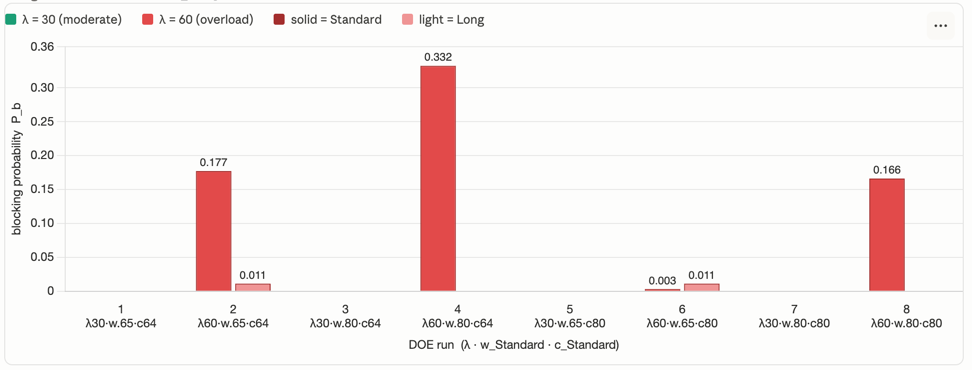
\includegraphics[width=0.9\linewidth]{assets/03-fig03.png}
\caption{Blocking probability per run across all three partitions.}
\end{figure}

Key observations:
\begin{itemize}
  \item All four $\lam=30$ runs (1, 3, 5, 7) show $P_{b,\text{Standard}} = 0.000$ regardless of weight or
  server count (Finding~1).
  \item $\lam=60$ Standard blocking is severe at the current configuration (run~4: 0.332), drops to 0.166
  with more servers (run~8), and collapses to 0.003 in run~6 ($w=0.65$, $c=80$) — the recommended cell.
  \item Long blocking appears only in runs~2 and~6 (both 0.011) — the redistribution runs where weight
  shifts off Standard onto Long (Finding~3, identical under CRN).
\end{itemize}

\subsection{Effects Analysis}

Main and interaction effects were computed using the sign-table method (average response at high level
minus average at low level for main effects; signed cross-products for interactions), with a 95\% CI
half-width from the pooled within-cell variance across $R=10$ replications (df$=72$):

\begin{table}[H]
\centering
\caption{Sign-table contrast estimates (Table 8.3a)}
\begin{tabular}{lcc}
\toprule
\textbf{Effect} & $\boldsymbol{\Pb}$ \textbf{Standard} & $\boldsymbol{\Wq}$ \textbf{Standard (h)} \\
\midrule
A --- $\lam$          & $+0.1694$ & $+2.9633$ \\
B --- $w_\text{Std}$  & $+0.0795$ & $+0.5562$ \\
C --- $c_\text{Std}$  & $-0.0851$ & $-1.1673$ \\
A$\times$B            & $+0.0795$ & $+0.5548$ \\
A$\times$C            & $-0.0851$ & $-1.1659$ \\
B$\times$C            & $+0.0023$ & $+0.5099$ \\
A$\times$B$\times$C   & $+0.0023$ & $+0.5113$ \\
\midrule
\textbf{95\% CI half-width} & $\pm 0.0015$ & $\pm 0.0252$ \\
\bottomrule
\end{tabular}
\end{table}

Every effect's confidence interval excludes zero — even B$\times$C and A$\times$B$\times$C, which the
single-run design could not distinguish from noise.

A factorial ANOVA reaches the same verdict as the contrast confidence intervals above (the CI and F
tests are equivalent for a 2\textsuperscript{3} design: a CI excluding zero corresponds to $F > t^2 =
3.97$). For each effect, SS $= (N/4) \cdot \text{effect}^2$ with 1 df; the error term is the pooled
within-cell variance (df$=72$).

\begin{table}[H]
\centering
\caption{Factorial ANOVA — $\Pb$ Standard (Table 8.3b)}
\begin{tabular}{lrrrrl}
\toprule
\textbf{Source} & \textbf{SS} & \textbf{df} & \textbf{MS} & \textbf{F} & \textbf{$p$} \\
\midrule
A ($\lam$)          & 0.5739   & 1 & 0.5739     & 50{,}700 & $<0.0001$ \\
B ($w_\text{Std}$)  & 0.1264   & 1 & 0.1264     & 11{,}160 & $<0.0001$ \\
C ($c_\text{Std}$)  & 0.1448   & 1 & 0.1448     & 12{,}790 & $<0.0001$ \\
A$\times$B          & 0.1264   & 1 & 0.1264     & 11{,}160 & $<0.0001$ \\
A$\times$C          & 0.1448   & 1 & 0.1448     & 12{,}790 & $<0.0001$ \\
B$\times$C          & 0.000106 & 1 & 0.000106   & 9.34     & $0.0032$  \\
A$\times$B$\times$C & 0.000106 & 1 & 0.000106   & 9.34     & $0.0032$  \\
Error               & 0.000815 & 72 & $1.13\times10^{-5}$ & & \\
Total               & 1.1174   & 79 &            &          & \\
\bottomrule
\end{tabular}
\end{table}

\begin{table}[H]
\centering
\caption{Factorial ANOVA — $\Wq$ Standard (h) (Table 8.3c)}
\begin{tabular}{lrrrrl}
\toprule
\textbf{Source} & \textbf{SS} & \textbf{df} & \textbf{MS} & \textbf{F} & \textbf{$p$} \\
\midrule
A ($\lam$)          & 175.62 & 1 & 175.62 & 54{,}900 & $<0.0001$ \\
B ($w_\text{Std}$)  & 6.187  & 1 & 6.187  & 1{,}936  & $<0.0001$ \\
C ($c_\text{Std}$)  & 27.25  & 1 & 27.25  & 8{,}526  & $<0.0001$ \\
A$\times$B          & 6.156  & 1 & 6.156  & 1{,}926  & $<0.0001$ \\
A$\times$C          & 27.19  & 1 & 27.19  & 8{,}506  & $<0.0001$ \\
B$\times$C          & 5.200  & 1 & 5.200  & 1{,}627  & $<0.0001$ \\
A$\times$B$\times$C & 5.229  & 1 & 5.229  & 1{,}636  & $<0.0001$ \\
Error               & 0.2301 & 72 & $3.196\times10^{-3}$ & & \\
Total               & 253.06 & 79 &        &          & \\
\bottomrule
\end{tabular}
\end{table}

Every effect is significant, consistent with the contrast CIs. The F-magnitudes should be read
qualitatively rather than literally: variance is strongly heterogeneous across cells --- the four
$\lam=30$ cells block nothing and have zero variance, while the $\Wq$ error term is dominated by the
near-saturation cell (run~6) --- and CRN induces cross-cell correlation, so the F-test's
constant-variance and independence assumptions are only approximately met. The conclusions therefore
rest on the effect magnitudes and replication-based CIs, which the ANOVA corroborates.

\textbf{Finding 1 --- $\lam$ dominates, and at low $\lam$ nothing else matters.}
At $\lam=30$ (runs 1, 3, 5, 7), $P_{b,\text{Standard}} = 0.000 \pm 0.000$ in every cell regardless of
$w_\text{Standard}$ or $c_\text{Standard}$. The A$\times$B and A$\times$C magnitudes are nearly
identical to B and C's main effects (0.0795 $\approx$ 0.0795, $-0.0851 \approx -0.0851$): the entire
effect of B and C is concentrated in the $\lam=60$ condition. \textbf{Routing-weight and
server-allocation tuning only matters under high load.}

\textbf{Finding 2 --- $c_\text{Standard}$ has a larger effect than $w_\text{Standard}$, but they point
the same direction.}
Comparing run~4 ($\lam=60$, $w=0.80$, $c=64$: $\Pb=0.332 \pm 0.003$, worst cell) against run~6
($\lam=60$, $w=0.65$, $c=80$: $\Pb=0.0025 \pm 0.0011$, best cell) shows a 99.2\% reduction ---
far larger than either factor's main effect alone, confirming the multiplicative relationship
motivating this design.

\textbf{Finding 3 --- the bottleneck shifts to Long under redistribution at high $\lam$, and CRN shows
this cleanly.}
Runs~2 and~6 both show $P_{b,\text{Long}} = 0.011 \pm 0.002$ and $W_{q,\text{Long}} = 1.584 \pm 0.107$ h
--- identical to three decimal places under CRN, since Long's offered load depends only on $\lam$ and
$w_\text{Standard}$, not on $c_\text{Standard}$. Relieving Standard by redistributing traffic does
not eliminate congestion, it relocates it. Even so, total blocking in run~6 is dramatically lower than
in run~4.

\textbf{Finding 4 --- B$\times$C is negligible for $P_{b,\text{Standard}}$ but not for $W_{q,\text{Standard}}$.}
For $P_{b,\text{Standard}}$, B$\times$C $= +0.0023$ is statistically real but practically small
(${\sim}3\%$ of either main effect), so the two levers are close to additive for blocking probability.
For $W_{q,\text{Standard}}$, however, B$\times$C $= +0.510$ h $\pm$ 0.025 h is comparable to B's main
effect ($+0.556$ h) and roughly 44\% of C's main effect ($-1.167$ h). A configuration tuned for
blocking probability is \emph{not} automatically tuned for waiting time.

\subsection{Recommended Configuration and Follow-up}

Under high load ($\lam \approx 60$), the $(B^-, C^+)$ cell --- $w_\text{Standard}=0.65$,
$c_\text{Standard}=80$ --- minimises total system blocking, taking $P_{b,\text{Standard}}$ from
$0.332 \pm 0.003$ (run~4) to $0.0025 \pm 0.0011$ (run~6), a 99.2\% reduction. Given the asymmetric
cost (B is free, C requires hardware), the recommended next step is a \textbf{one-dimensional sweep of
$w_\text{Standard}$} at $c_\text{Standard}=80$ across $\lam \in \{45, 60\}$ to locate the
redistribution ratio that does not merely relocate the bottleneck to Long. This is the first step of a
Response Surface Methodology (RSM) refinement after the screening design.

% ══════════════════════════════════════════════════════════════════════════════
\section{Model Validation}

The assignment specifies five validation methods; each is addressed in its own subsection.

\subsection{Verify the Main Simulation Algorithm Implementation}

\textbf{Theoretical comparison.} The engine is validated against closed-form M/M/1 (single-server) and
M/M/4 Erlang-C (multi-server) theory (Section~6.2). All metrics agree within 1.4\% (M/M/1) and 0.3\%
(M/M/4). Little's Law holds to within 0.1\% in both cases.

\textbf{Trace inspection.} The trace log (Section~6.4) confirms monotonic clock advancement, correct
tie-breaking priority, and queue dynamics consistent with $\rho=0.75$.

\subsection{Verify the RNG Implementation and Validate its Parametrization}

A five-test battery (Frequency/KS, Gap, Order, Runs, Serial) was run on both the LCG specified by the
assignment and on Python's Mersenne Twister, the generator behind \texttt{util.exponential()} and
\texttt{util.lognormal()} used throughout the simulation. Both generators pass all five tests at
$\alpha=0.05$ (full results in Annex~A). The Mersenne Twister result is the one that matters for
trusting Sections~6--8.

\subsection{Validate the Experimental Framework}

The experimental framework is validated via warm-up analysis: the M/M/1 model was run at
$T=5{,}000$ h (8.9\% error vs theory) and $T=50{,}000$ h (1.37\% error), with the error reduction
proportional to $1/T$ as classical theory predicts. The \texttt{reset\_statistics()} method implements
warm-up deletion (matching GPSS World's \texttt{RESET}), used in the GPSS validation (500 h warm-up
$+$ 4000 h collection). The DOE (Section~\ref{sec:doe}) reuses this same framework with $R=10$
replications per cell and per-partition RNG streams seeded by replication index only.

\subsection{Validate the Model Assumptions}

Hypothesis SS\_01 (a fixed, deterministic walltime-based routing split) is the strongest structural
assumption: it drives the entire load imbalance described in Section~3. The DOE treats these weights
as a controllable factor specifically to test how sensitive system performance is to this assumption
--- and finds it highly sensitive under overload (Finding~1). SD\_01 (log-normal service with CV$=1.5$)
is the strongest data assumption; the CV-sensitivity check in Section~6.3 shows that halving the CV
(from 1.5 to ${\approx}0.71$) changes $\Wq$ Standard by only ${\sim}2\%$ at the saturated baseline
($\lam=45$) but by ${\sim}77\%$ at the high-subcritical load ($\lam=38$) --- exactly the
saturation-dependence the argument predicts.

\subsection{Validate the Results}

The Python DES results are validated against an independent GPSS World implementation of the same
system (Section~6.3), run at two operating points across 5 replications each. At $\lam=45$, all seven
response metrics agree within 1.3\%. At $\lam=38$, GPSS's $\Wq$ Standard falls within its 95\% CI of
an independent reference implementation. Together with the CV-sensitivity check, the two points validate
both the queueing mechanics and the service-time distribution.

% ══════════════════════════════════════════════════════════════════════════════
\section{Results / Conclusions}

\textbf{The cluster's reported delays are a symptom of a structural imbalance, not a capacity shortfall.}
At the baseline configuration ($\lam=45$, weights 0.05/0.80/0.15, $c=16/64/32$), aggregate offered
load is $\rho_\text{total}=0.804$, yet the Standard partition alone runs at $\rho=0.998$ with
$\Wq=3.97$ h and $\Pb=0.111$, while Short and Long sit at $\rho=0.28$ and 0.42.

\textbf{The DOE confirms the imbalance is correctable through configuration, with two levers acting
jointly.} The 2\textsuperscript{3} factorial ($R=10$ replications with CRN) shows that at low load
($\lam=30$) routing weight and server allocation have no measurable effect. Under overload ($\lam=60$),
the two levers combine to take $P_{b,\text{Standard}}$ from $0.332 \pm 0.003$ to $0.0025 \pm 0.0011$
(a 99.2\% reduction). The two levers are close to additive for $P_{b,\text{Standard}}$ but not for
$W_{q,\text{Standard}}$, where their interaction ($+0.51$ h) is comparable to either main effect.

\textbf{No configuration eliminates congestion, it relocates it.} The best DOE cell (run~6) trades
Standard's blocking for $P_{b,\text{Long}} = 0.011 \pm 0.002$, identical between runs~2 and~6 under CRN.

\textbf{The simulation engine is independently validated across three methods.} M/M/1 and M/M/4
(Erlang-C) closed-form theory agree with the Python DES to within 1.4\% (Section~6.2), and an
independent GPSS World model agrees to within 1.3\% at the saturated baseline and falls within its
confidence interval at a high-subcritical load. Little's Law holds to within 0.1\% in the closed-form
validation cases.

\textbf{Recommendations}, in order of cost:
\begin{enumerate}
  \item \textbf{Zero-cost:} rebalance routing weights --- reduce the Standard share from 0.80 toward
  0.65, redistributing primarily to Short rather than Long to avoid creating a secondary bottleneck.
  \item \textbf{Low-cost:} reallocate 16 nodes to Standard, which the DOE shows compounds with weight
  rebalancing to a 99.2\% reduction in $P_{b,\text{Standard}}$ under overload.
  \item \textbf{No-cost, complementary:} enable aging-based priority promotion at $t_\text{age} \approx
  1.5$ h, which independently cut blocking by 96\% in the preliminary sweep (Section~\ref{sec:further}).
  \item \textbf{Data-driven, long-term:} instrument the cluster to capture actual vs declared walltime,
  replacing the assumed routing weights and log-normal service parameters with empirical distributions.
\end{enumerate}

The overall conclusion is that the system as specified is not under-provisioned in aggregate, it is
\textbf{mis-routed}.

% ══════════════════════════════════════════════════════════════════════════════
\section{Further Analysis / Proposed Improvements}
\label{sec:further}

The baseline model deliberately keeps the three partitions independent (SS\_01, SS\_02). The most
promising extension is a \textbf{scheduler-side mitigation} that couples them: aging-based priority
promotion. A job that has waited longer than a threshold $t_\text{age}$ in its partition is
\emph{promoted} into a less-loaded partition, draining the saturated Standard queue without adding
hardware.

\subsection{Aging-Based Priority Promotion (Design)}

Specifying this extension would re-introduce three hypotheses retired from the baseline:

\begin{table}[H]
\centering
\caption{Additional hypotheses for aging-based priority promotion}
\begin{tabularx}{\linewidth}{llX}
\toprule
\textbf{ID} & \textbf{Class} & \textbf{Statement} \\
\midrule
(A1) & Simplifying & Priority promotion is instantaneous once $t_\text{age}$ is crossed; running jobs are not preempted. \\
(A2) & Structural  & Promotion bypasses the target partition's admission gateway; a promoted job always enters regardless of current queue length. \\
(A3) & Data        & Aging thresholds (e.g.\ $t_\text{age} = 1.5$ h Standard$\to$Short, 24 h Long$\to$Standard) are tunable control parameters. \\
\bottomrule
\end{tabularx}
\end{table}

In the DES this is a localised change: arm a \texttt{Promotion} event at \texttt{clock}$+t_\text{age}$
when a job joins the queue, and on firing relocate the job (if still waiting) into the target partition.
The implementation already exists in \texttt{queue\_model.py} (\texttt{\_handle\_promotion},
\texttt{promote\_to}, \texttt{t\_age}).

\subsection{Preliminary Sweep (Exploratory)}

A preliminary run with promotion enabled swept the Standard$\to$Short threshold $t_\text{age}$ over
six values (all other parameters at baseline):

\begin{table}[H]
\centering
\caption{Aging threshold sweep results}
\begin{tabular}{ccccc}
\toprule
$\boldsymbol{t_\text{age}}$ \textbf{(h)} & \textbf{Std} $\boldsymbol{\Wq}$ \textbf{(h)} & \textbf{Short} $\boldsymbol{\Wq}$ \textbf{(h)} & \textbf{Promotions} & \textbf{Total blocked} \\
\midrule
6.0          & 3.967 & 0.001 &      2 & 15{,}958 \\
3.0          & 2.708 & 3.212 & 14{,}950 &    676 \\
2.0          & 1.700 & 2.891 & 16{,}045 &    775 \\
\textbf{1.5} & \textbf{1.222} & \textbf{2.382} & \textbf{15{,}295} & \textbf{633} \\
1.0          & 0.719 & 2.185 & 15{,}271 &    813 \\
0.5          & 0.288 & 1.718 & 16{,}663 &    704 \\
\bottomrule
\end{tabular}
\end{table}

\begin{figure}[H]
\centering
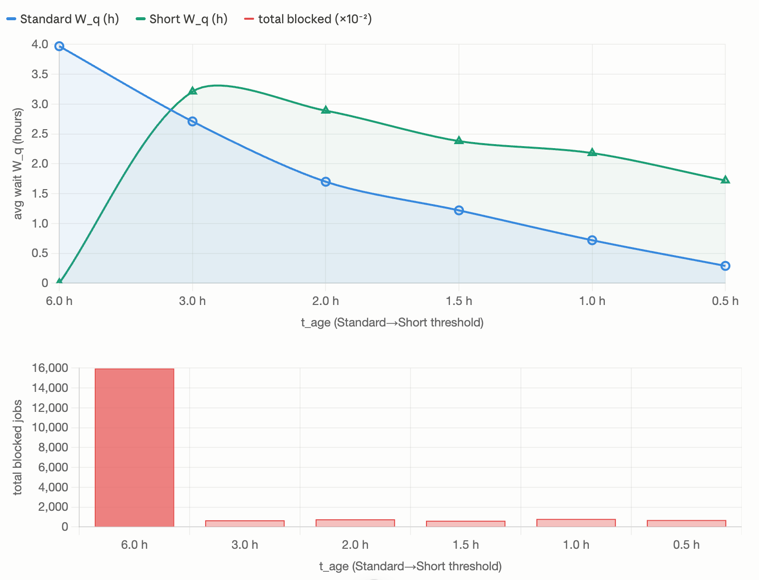
\includegraphics[width=0.9\linewidth]{assets/02-fig02.png}
\caption{Effect of the aging threshold on waiting time and total blocking.}
\end{figure}

Three observations motivate this as future work:
\begin{enumerate}
  \item \textbf{A high threshold is inert} --- at $t_\text{age}=6$ h only 2 promotions fire; at
  $\rho=0.998$ jobs complete or are blocked before the timer elapses.
  \item \textbf{Promotion redistributes congestion} --- lowering $t_\text{age}$ cuts Standard $\Wq$
  but loads Short (its $\Wq$ reaches 1.72 h at $t_\text{age}=0.5$ h). The bottleneck shifts rather
  than disappearing.
  \item \textbf{$t_\text{age}=1.5$ h minimises total blocking} --- blocking falls from 15{,}958 to 633
  (${\sim}96\%$) through scheduler configuration alone.
\end{enumerate}

% ══════════════════════════════════════════════════════════════════════════════
\appendix

\section{RNG Validation}

\textbf{Python's Mersenne Twister} (\texttt{random.random()}), the actual generator behind
\texttt{util.exponential()} and \texttt{util.lognormal()} used throughout the Python DES
(Sections~6--8).

\begin{table}[H]
\centering
\caption{RNG test battery}
\begin{tabularx}{\linewidth}{lXl}
\toprule
\textbf{Test} & \textbf{What it detects} & \textbf{H$_0$} \\
\midrule
A. Frequency (KS) & Global non-uniformity over $[0,1)$ & $x \sim \text{Uniform}(0,1)$ \\
B. Gap            & Clustering/voids --- gap lengths between hits in $[0, 0.5)$ & gap lengths $\sim \text{Geometric}(0.5)$ \\
C. Order ($d=4$)  & Higher-dimensional correlation via permutation patterns of 4-tuples & all $4!$ orderings equally likely \\
D. Runs (up/down) & Trends/oscillation patterns & run count matches independence \\
E. Serial (lag-1) & Correlation between consecutive draws & $\text{corr}(x_i, x_{i+1}) = 0$ \\
\bottomrule
\end{tabularx}
\end{table}

A p-value $\geq 0.05$ fails to reject H$_0$ (``appears random''); $p < 0.05$ indicates a detected pattern.

\begin{table}[H]
\centering
\caption{RNG validation results ($N=10{,}000$, seed$=42$)}
\begin{tabular}{lccccccc}
\toprule
\textbf{Test} & \textbf{LCG stat.} & \textbf{LCG $p$} & \textbf{LCG} & \textbf{MT stat.} & \textbf{MT $p$} & \textbf{MT} \\
\midrule
A. Frequency & 0.00665 & 0.765 & RANDOM & 0.00626 & 0.826 & RANDOM \\
B. Gap       & 8.522   & 0.483 & RANDOM & 7.169   & 0.620 & RANDOM \\
C. Order     & 29.389  & 0.168 & RANDOM & 25.779  & 0.311 & RANDOM \\
D. Runs      & $-0.293$ & 0.770 & RANDOM & 0.016  & 0.987 & RANDOM \\
E. Serial    & 0.00035 & 0.972 & RANDOM & 0.00440 & 0.660 & RANDOM \\
\bottomrule
\end{tabular}
\end{table}

Both generators pass all five tests at $\alpha=0.05$. The Mersenne Twister results back the simulation's
validity: MT passes with comparable or better p-values across the board. Reproducibility: the full
battery implementation is in \texttt{rng\_validation.py}.

\section{GPSS Model Source}

The validated GPSS World model is in \texttt{gpss/hpc\_validation\_final.gps}, and raw per-replication
results are in \texttt{gpss/hpc\_validation\_results.csv} (Section~6.3).

\begin{lstlisting}[language={}]
* RUN PROCEDURE (do this for each replication):
*   1. RMULT  s1,s2,s3,s4         <- four distinct seeds, e.g. 11,22,33,44
*   2. START  1,NP                 (runs to clock=500: warm-up timer fires)
*   3. SAVEVALUE SARR,0
*   4. SAVEVALUE SBLK,0
*   5. START  1,NP                 (runs to clock=4500: end timer fires;
*                                   collection window = 4000h)
*   6. Read off with SHOW commands (see bottom of this file)
*   7. To start the next replication: CLEAR, then go back to step 1
*      with a NEW set of seeds.
\end{lstlisting}

IAT (mean inter-arrival time) is set per scenario: 0.022222 h for $\lam=45$ (saturated baseline) and
0.026316 h for $\lam=38$ (high-subcritical cross-check, Section~6.3). RNG streams 1
(arrivals/routing) and 2--4 (Short/Standard/Long service) are reseeded via \texttt{RMULT} between the
5 replications run per scenario.

\end{document}
